\documentclass{article}
\usepackage{amsmath}
\usepackage{amssymb}
\usepackage{tikz}
\usetikzlibrary{patterns,decorations.pathreplacing}
\usepackage{xcolor}

\begin{document}

    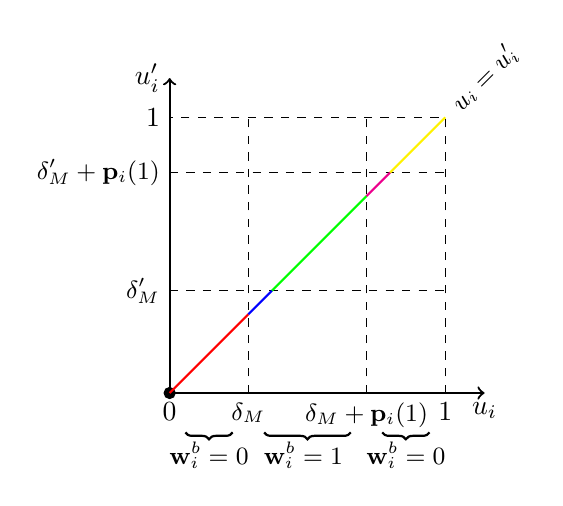
\begin{tikzpicture}
    \draw[thick,<->] (4,0) -- (0,0) -- (0,4);
    \filldraw[black] (0,0) circle (2pt) node[anchor=north]{0};
    \node [left] at (0,4) {$u^{\prime}_{i}$};
    \node [below] at (4,0){$u_i$};
    \draw[dashed] (3.5,0) -- (3.5,3.5) -- (0,3.5);
    \node [below] at (3.5,0){1};
    \node [left] at (0,3.5){1};
    \draw[dashed] (1,0) -- (1,3.5);
    \node [below] at (1,0){\small{$\delta_M$}};
    \draw[dashed] (2.5,0) -- (2.5,3.5);
    \node [below] at (2.5,0){\small{$\delta_M +\mathbf{p}_i(1)$}};
    \draw[dashed] (0,1.3) -- (3.5,1.3);
    \node [left] at (0,1.3){\small{$\delta^{\prime}_M$}};
    \draw[dashed] (0,2.8) -- (3.5,2.8);
    \node [left] at (0,2.8){\small{$\delta^{\prime}_M + \mathbf{p}_i(1)$}};
    \draw [thick,red](0,0) -- (1, 1);
    \draw [thick,blue](1,1) -- (1.3, 1.3);
    \draw [thick,green](1.3,1.3) -- (2.5, 2.5);
    \draw [thick,magenta](2.5,2.5) -- (2.8, 2.8);
    \draw [thick,yellow](2.8,2.8) -- (3.5, 3.5);
    \node [rotate = 45] at (4,4){\small{$u_i = u^{\prime}_i$}};
    \draw [decorate,decoration = {brace, mirror}, thick] (0.2,-0.5) --  (0.8,-0.5);
    \node [below] at (0.5,-0.5) {\small{$\mathbf{w}^b_i = 0 $}};
    \draw [decorate,decoration = {brace, mirror}, thick] (1.2,-0.5) --  (2.3,-0.5);
    \node [below] at (1.7,-0.5) {\small{$\mathbf{w}^b_i = 1 $}};
    \draw [decorate,decoration = {brace, mirror}, thick] (2.7,-0.5) --  (3.3,-0.5);
    \node [below] at (3,-0.5) {\small{$\mathbf{w}^b_i = 0 $}};
\end{tikzpicture}

\end{document}